
\documentclass{../concepts/titul_protokol_p/prepareprotokol} %všechny balíčky pro protokol + titulní strana

\usepackage{graphicx}
\usepackage{newfloat}
\usepackage{caption}
\usepackage{booktabs}
\usepackage{amssymb}
\usepackage{amsmath}
\usepackage{siunitx}
\usepackage{textcomp}
\usepackage{comment}
\usepackage{gensymb}
\usepackage{subcaption}
\usepackage{multirow}
\sisetup{inter-unit-product =$\cdot$}
%\sisetup{separate-uncertainty=true}

\praktikum{III} %číslo praktika (I, II nebo III)
\autor{David Němec} %jméno autora
\datum{24.\,3.\,2026} %datum měření
\cislo{9} %číslo úlohy
\nazev{Měření indexu lomu dvouhranolovým a polokulovým refraktometrem} %název úlohy

\DeclareFloatingEnvironment[fileext=los, placement={htbp}, name=Obrázek]{schema}

\newcommand{\nobars}{
Chybové úsečky nebyly pro~svou malou velikost pro~přehlednost vykresleny.}

\newcommand{\relative}[1]{
\frac{\sigma_{#1}}{#1}
}
\newcommand{\squared}[1]{
\left( #1 \right)^2
}
\newcommand{\relsqr}[1]{
\squared{\relative{#1}}
%\left( \frac{\sigma_{#1}}{#1} \right)^2
}

\begin{document}
\renewcommand{\figurename}{Graf}
\renewcommand{\refname}{Literatura}
\renewcommand{\today}{\number\day.\,\number\month.\,\number\year}

% add another graphics path to find ZPF.pdf for title page
% now searches for images in ./ and ../concepts/titul_protokol_p/
\graphicspath{{../concepts/titul_protokol_p/}}
\maketitle

% ========================== PRACOVNÍ ÚKOL ============================
\section{Pracovní úkol}
\begin{enumerate}
    \item Změřte index lomu a střední disperzi přiložené kapaliny v závislosti na koncentraci (stačí 5 různých koncentrací).
    \item Změřte indexy lomu tří optických skel:
    \begin{enumerate}
        \item vzorek s daným indexem lomu,
        \item simax nebo pyrex,
        \item jeden z očíslovaných kvádrů z krabičky „vzorky skel“.
    \end{enumerate}
    \item Změřte index lomu řádného paprsku a index lomu mimořádného paprsku přiloženého dvojlomného materiálu v závislosti na směru šíření světla.
    \item Z měření v bodu 3. stanovte, zda jde o kladný či záporný jednoosý krystal.
    \item U všech naměřených hodnot indexu lomu určete chybu nepřímého měření.
\end{enumerate}

% ============================= TEORIE ================================
\section{Teorie}
\subsection{Zákon odrazu a lomu světla, mezní úhel}
Při dopadu paprsku světla na~rozhraní dvou prostředí pod úhlem $\alpha_1$ (měřeným mezi normálou k~rozhraní
a~směrem paprsku) se~paprsek částečně odráží a~částečně láme. Odražený i~lomený paprsek leží v~rovině dopadu,
která je daná normálou k~rozhraní a~směrem dopadajícího paprsku. Podle zákona odrazu platí, že úhel
odrazu $\alpha_1'$ je rovný úhlu dopadu $\alpha_1$ \cite{studijni}. Podle zákona lomu závisí úhel lomu
$\alpha_t$ na~úhlu dopadu, ale i~na~indexech lomu obou prostředí $N_1$ a~$N_2$, a~to podle vztahu \cite{studijni}
\begin{equation}
    \label{eq:snell}
    N_1 \sin \alpha_1 = N_2 \sin \alpha_2 \,.
\end{equation}

Při chodu paprsku z~opticky hustšího do~opticky řidšího prostředí ($N_1 > N_2$) existuje mezní úhel
$\alpha_m$, pro~který je~úhel lomu $\alpha_2$ roven $90 \,\degree$. Pro~úhly dopadu větší než~mezní úhel již
nedochází k~lomu, ale~k~totálnímu odrazu paprsku. Rovnice (\ref{eq:snell}) pak přejde na~tvar \cite{studijni}
\begin{equation}
    \label{eq:mezni}
    \sin \alpha_m = \frac{N_2}{N_1} \,.
\end{equation}

% =================================
\subsection{Měření indexu lomu dvouhranolovým refraktometrem}

Schéma dvouhranolového refraktometru je~zobrazeno na~obrázku \ref{sch:dvouhranolovy}. Bílé světlo prochází
stěnou QR do~soustavy hranolů $\mathrm{H_1}$ a $\mathrm{H_2}$, mezi nimiž je~vrstva studované kapaliny K
o~indexu lomu menším než~index lomu hranolu $\mathrm{H_1}$.
Světlo rozptýlené na~zdrsněné ploše PR vstupuje do~kapaliny pod~všemi úhly, pro~úhly větší než~mezní úhel
$\alpha_m$ však dochází k~totálnímu odrazu, takže tyto paprsky se~nelámou a~nepostupují dále měřicí soustavou.
Díky nepřítomnosti paprsků s~úhlem dopadu větším než $\alpha_m$ lze~v~dalekohledu následně pozorovat rozhraní
světlo-stín. U~většiny komerčních refraktometrů lze~na~stupnici S přímo odečítat indexy lomu vzorku kapaliny K.

\begin{schema}[htbp]
    \centering
    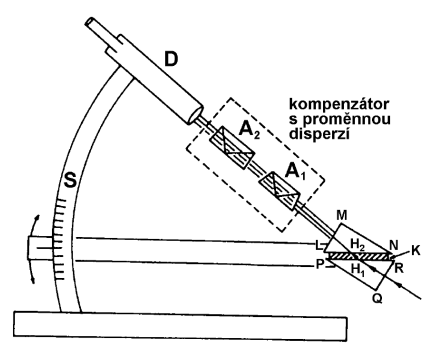
\includegraphics[width=0.5\linewidth]{dvouhranolovy.png}
    \caption{Schéma dvouhranolového refraktometru \cite{pokyny}}
    \label{sch:dvouhranolovy}
\end{schema}

Mezní úhel však kvůli disperzi závisí na~vlnové délce, což při měření s bílým světlem způsobí neostrost
a~barevnost tohoto rozhranní. Proto je potřeba meřicí soustavu vybavit kompenzátorem, jež má disperzi
přesně opačnou než soustava hranolů $\mathrm{H_1}$ a $\mathrm{H_2}$ s~kapalinou K. K~tomu se~využívá
soustava dvou Amiciho hranolů (schéma na obr. \ref{sch:amici}), jejichž vzájemným pootočením lze vhodně
nastavit velikost odchylky paprsků C a F, a tím i disperze tohoto kompenzátoru. Ze~znalosti závislosti disperze
kompenzátoru na~vzájemném otočení Amiciho hranolů a~disperze samotné soustavy $\mathrm{H_1}$-$\mathrm{H_2}$
lze takto určit střední disperzi $\Delta$ kapaliny K.

\begin{schema}[htbp]
    \centering
    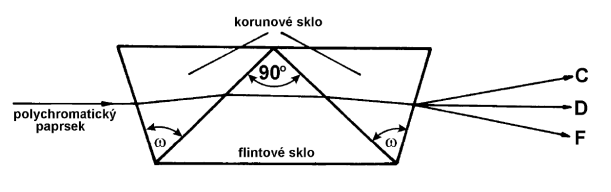
\includegraphics[width=0.5\linewidth]{amici.png}
    \caption{Amiciho přímohledný hranol \cite{pokyny}}
    \label{sch:amici}
\end{schema}

% =================================
\subsection{Měření indexu lomu polokulovým refraktometrem}
Schéma polokulového refraktometru je na~obrázku \ref{sch:polokulovy}, přičemž měření probíhalo v~odraženém
světle, tedy se~směrem paprsků \textbf{(2)}. Světlo ze~sodíkové výbojky s~maximem intenzity pro~vlnovou
délku $\lambda_\mathrm{Na} = \qty{589.3}{nm}$ \cite{vlnovedelky} se~(pro snadnější manipulaci) odráží
od~zrcátka a~dopadá na~skleněnou polokouli o~indexu lomu $N_1$ pod~různými úhly $\alpha$. Na~horní stěně
polokoule je umístěn zkoumaný vzorek s~indexem lomu $N_2$, přičemž mezi ním a~polokoulí je (pro zajištění
optického kontaktu) tenká vrstva imerzní kapaliny s~takový indexem lomu $N_i$, aby platilo $N_1 > N_i > N_2$.
V~tomto případě byl použit monobromnaftalen s~$N_i = 1.658$ \cite{pokyny}. 

Díky faktu, že $N_1 > N_2$, dochází
na~horní stěně koule k~totálnímu odrazu jen těch paprsků s~úhlem dopadu $\alpha > \alpha_m$. Ostatní se~lámou
a~vystupují ven z~optické soustavy, díky čemuž bude jejich intenzita v~dalekohledu D nižší než u~totálně odražených
paprsků. V~dalekohledu tak bude pozorovatelné ostré rozhraní světlo-polostín a~díky zákonu odrazu lze ze~sklonu
dalekohledu určit mezní úhel $\alpha_m$. Pokud označím $\alpha_{m0}$ mezní úhel samotné polokoule 
(kdy druhé prostředí je vzduch, $N_2 = 1$), lze pro~tyto dvě situace se~vzorkem a~bez vzorku z~rovnice
(\ref{eq:mezni}) odvodit vztah pro~index lomu vzorku $N_2$ \cite{pokyny}:
\begin{equation}
    \label{eq:indexvzorku}
    N_2 = N_1 \sin \alpha_m = \frac{\sin \alpha_m}{\sin \alpha_{m0}} \,.
\end{equation}

\begin{schema}
    \centering
    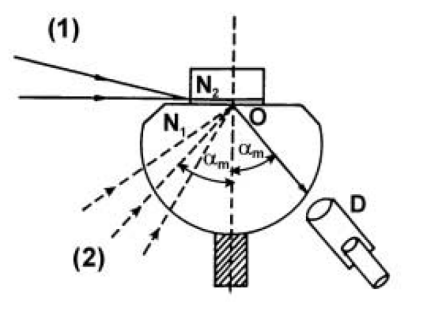
\includegraphics[width=0.5\linewidth]{polokulovy.png}
    \caption{Abbeův polokulový refraktometr \cite{pokyny}}
    \label{sch:polokulovy}
\end{schema}

% =================================
\subsection{Měřicí přístroje a jejich nejistoty}
\begin{enumerate}
    \item \textbf{Refraktometr Novex}:
    
    Pomocí refraktometru Novex byl měřen index lomu a střední disperze roztoku glukózy. Nejistotu určení indexu
    lomu (nejistota tybu B) odhaduji jako velikost nejmenšího dílku stupnice, tedy $\sigma_{N,B}= 5\cdot10^{-4}$.
    Nejistotu určení pozice Amiciho hranolů vůči sobě odhaduji jako polovinu nejmenšího dílku
    stupnice, tedy $\sigma_Z = 0.5$.

    \item \textbf{Abbeův polokulový refraktometr}:

    Polokulovým refraktometrem byl měřen index lomu použité polokoule, dvou optických skel, simaxu a~křemene.
    Nejistotu pozice dalekohledu vůči dělené stupnici odhaduji jako velikost nejmenšího dílku
    stupnice, tedy $\sigma_{\alpha,B} = 1'$ (jedna úhlová minuta). Nejistotu otočení polokoule okolo svislé
    osy odhaduji jako $\sigma_{\varphi} = 2 \,\degree$, i~když stupnice umožnovala odečítat úhly jen~s~přesností
    $5\,\degree$.

\end{enumerate}


% ======================== VÝSLEDKY MĚŘENÍ ===========================
\section{Výsledky měření}

% ================================ chybí disperze na koncentraci
\subsection{Indexu lomu a střední disperze roztoku glukózy}

Měření bylo prováděno s~dvouhranolovým refraktometrem Novex, jež byl osvětlován bílým světlem.
Ze~zásobního roztoku glukózy o~koncentraci $c_m = \qty{500}{g \per l}$ bylo připraveno 5 vzorků
o~koncentracích $\qty{100}{g \per l}$, $\qty{200}{g \per l}$, $\qty{300}{g \per l}$, 
$\qty{400}{g \per l}$, $\qty{500}{g \per l}$ a jeden vzorek čisté destilované vody. Předpokládám, 
že~zásobní roztok měl objemovou koncentraci $100\,\%$, proměřované vzorky mají tedy objemové koncentrace
$0\,\%$, $20\,\%$, $40\,\%$, $60\,\%$, $80\,\%$ a~$100\,\%$. Pro~každý vzorek byla provedena tři měření
indexu lomu a~střední disperze (natočení Amiciho hranolů vůči sobě), z nichž byl následně vypočítán průměr
a~jeho směrodatná odchylka (nejistota typu A) podle vztahu \cite{englich}:
\begin{equation}
    \label{eq:glukoza_sigma_prumer_n}
    \sigma_{\overline{N},A} = \sqrt{\frac{\sum_{i=1}^{3} (N_i - \overline{N})}{6}} \,,
\end{equation}
kde $N_i$ jsou~naměřené hodnoty indexu lomu a~$\overline{N}$ je~jejich průměr. Nejistota indexu lomu byla
následně upravena o~nejistotu typu B $\sigma_{N,B} = 5\cdot10^{-4}$ podle vztahu \cite{englich}:
\begin{equation}
    \label{eq:glukoza_sigma_n}
    \sigma_{N} = \sqrt{\sigma_{\overline{N},A}^2 + \sigma_{N,B}^2} \,.
\end{equation}

Během měření byla kontinuálně
zaznamenávána teplota, všechny její hodnoty společně s~indexem lomu v~závislosti na~koncentraci vzorku
jsou v~tabulce \ref{tab:glukoza_indexy}.

\begin{table}[!htbp]
\centering
\caption{Index lomu a teplota okolí během měření roztoků glukózy o~různých koncentracích}
\begin{tabular}{ccc}
 \toprule
 $c\, (\mathrm{\%})$ & $N_D$ & $t\, (\mathrm{\degree C})$ \\
 \midrule
  \multirow{3}{*}{$0$} & $1.3320(5)$ & $23.5(4)$ \\
  & $1.3310(5)$ & $23.5(4)$ \\
  & $1.3315(5)$ & $23.5(4)$ \\
 \midrule
 \multirow{3}{*}{$20$} & $1.3450(5)$ & $23.6(4)$ \\
 & $1.3455(5)$ & $23.5(4)$ \\
 & $1.3450(5)$ & $23.6(4)$ \\
 \midrule
 \multirow{3}{*}{$40$} & $1.3535(5)$ & $23.8(4)$ \\
 & $1.3530(5)$ & $23.8(4)$ \\
 & $1.3535(5)$ & $23.9(4)$ \\
 \midrule
 \multirow{3}{*}{$60$} & $1.3660(5)$ & $23.9(4)$ \\
 & $1.3660(5)$ & $24.0(4)$ \\
 & $1.3665(5)$ & $24.0(4)$ \\
 \midrule
 \multirow{3}{*}{$80$} & $1.3750(5)$ & $24.0(4)$ \\
 & $1.3750(5)$ & $24.0(4)$ \\
 & $1.3750(5)$ & $24.0(4)$ \\
 \midrule
 \multirow{3}{*}{$100$} & $1.3890(5)$ & $24.0(4)$ \\
 & $1.3885(5)$ & $24.0(4)$ \\
 & $1.3885(5)$ & $24.0(4)$ \\
 \bottomrule
\end{tabular}
\label{tab:glukoza_indexy}
\end{table}

Jelikož byla hodnota pozice Amiciho hranolů $Z$ kromě jednoho měření pro~všechny vzorky stejná a~hodnoty 
jsou v~tabulce pro~výpočet disperze uvedeny s~přesností pouze na~jednotky, uvažuji konstantní hodnotu 
$Z = 42.0(5)$ pro~všechny vzorky. Z~ní byla podle tabulky \cite{novex} určena hodnota parametru
$\sigma = -0.59(2)$. Protože nejistu pozice hranolů $Z$ uvažuji $\sigma_Z = 0.5$, bude nejistota 
parametru $\sigma$ rovna polovině rozdílu hodnot v~tabulce, které sousedí s~touto
hodnotou, tedy polovině rozdílu $|\sigma_{Z=42} - \sigma_{Z=41}|$ případně rozdílu $|\sigma_{Z=43} - \sigma_{Z=42}|$
oba totiž po~zaokrouhlení na~jednu platnou číslici vycházejí stejně. Společně s parametry $A$ a~$B$
(danými z~tabulky \cite{novex} indexem lomu vzorku) vystupuje parametr $\sigma$
ve~vztahu pro~výpočet střední disperze \cite{novex}:
\begin{equation}
    \label{eq:delta}
    \Delta = A + \sigma \cdot B \,.
\end{equation}
Nejistota střední disperze byla vypočítána podle \cite{englich} jako
\begin{equation}
    \label{eq:sigma_delta}
    \sigma_\Delta = B \sigma_\sigma \,,
\end{equation}
přičemž nejistoty parametrů $A$ a~$B$ jsou díky přesnému měření indexu lomu vůči nejistotě parametru
$\sigma$ zanedbatelné. Hodnoty indexu lomu, parametrů $A$, $B$, teploty a střední disperze v~závislosti
na koncentraci vzorku jsou uvedeny v~tabulce \ref{tab:glukoza_vsechno}. Závislost indexu lomu
a~střední disperze na~koncentraci jsou také vykresleny v~grafech \ref{fig:glukoza_n} a~\ref{fig:glukoza_delta}.

\begin{table}[!htbp]
\centering
\caption{Index lomu, odpovídající parametry pro~výpočet střední disperze, střední disperze a~teplota
roztoku během měření pro~různě koncentrované roztoky.}
\begin{tabular}{cccccc}
 \toprule
 $c\, (\mathrm{\%})$ & $N_D$ & $A$ & $B$ & $\Delta$ & $t\, (\mathrm{\degree C})$ \\
 \midrule
 $0$ & $1.3315(6)$ & $0.02484$ & $0.03304$ & $0.0054(7)$ & $23.5(4)$ \\
 $20$ & $1.3452(5)$ & $0.02474$ & $0.03265$ & $0.0055(7)$ & $23.6(4)$ \\
 $40$ & $1.3533(5)$ & $0.02474$ & $0.03265$ & $0.0055(7)$ & $23.8(4)$ \\
 $60$ & $1.3662(5)$ & $0.02466$ & $0.03221$ & $0.0057(6)$ & $24.0(4)$ \\
 $80$ & $1.3750(5)$ & $0.02461$ & $0.03197$ & $0.0058(6)$ & $24.0(4)$ \\
 $100$ & $1.3887(5)$ & $0.02457$ & $0.03170$ & $0.0059(6)$ & $24.0(4)$ \\
 \bottomrule
\end{tabular}
\label{tab:glukoza_vsechno}
\end{table}

\begin{figure}[!htbp]
    \centering
    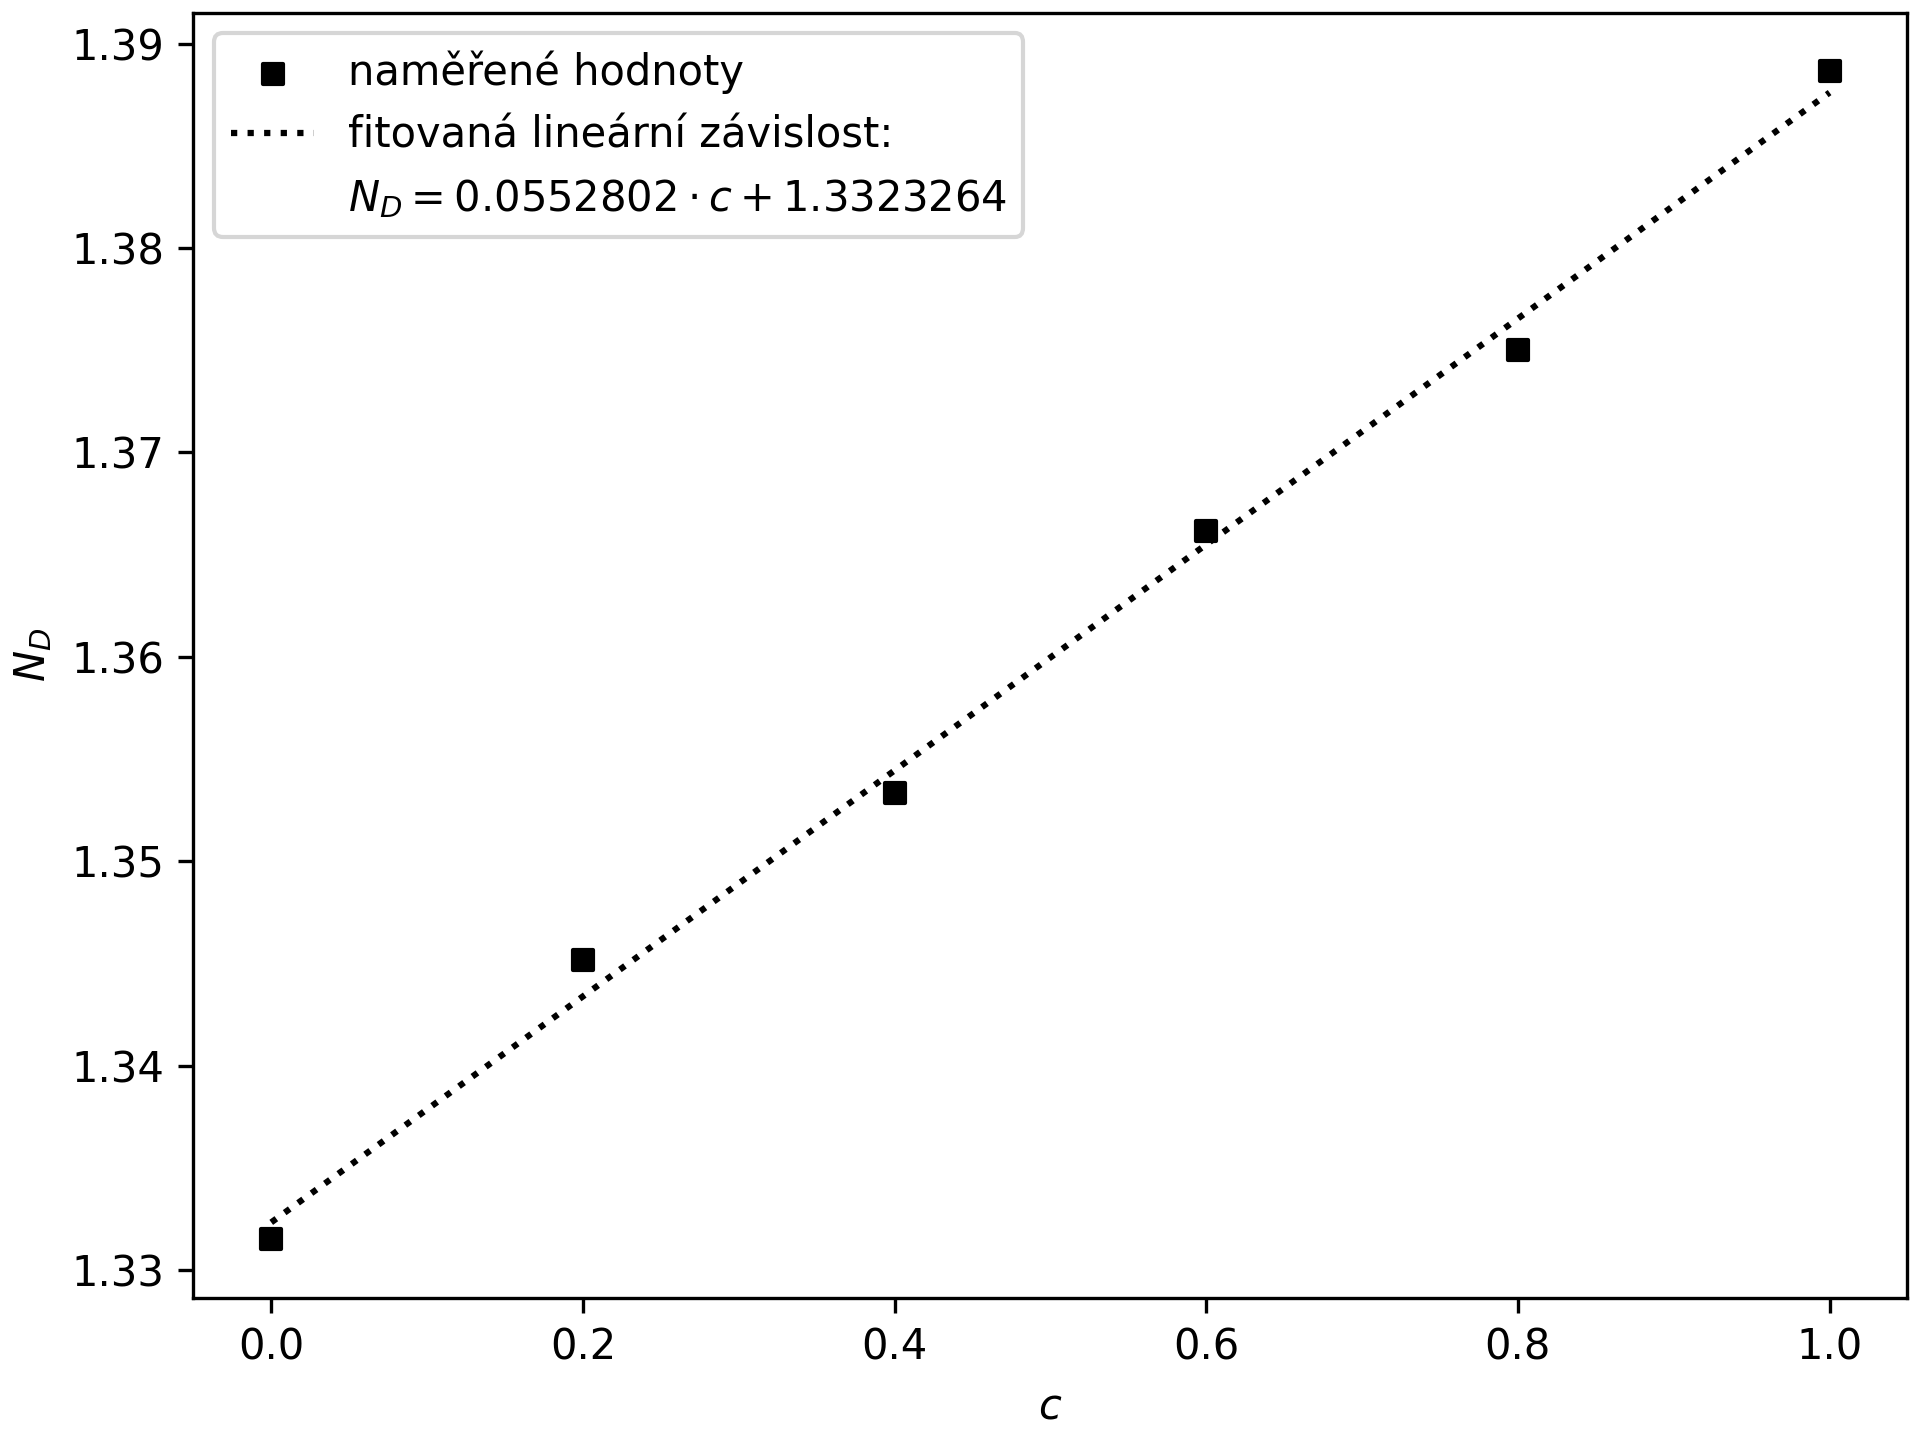
\includegraphics[width=0.5\linewidth]{glukoza_n.png}
    \caption{Závislost indexu lomu roztoku glukózy na~koncentraci vzorku.\nobars}
    \label{fig:glukoza_n}
\end{figure}

\begin{figure}[!htbp]
    \centering
    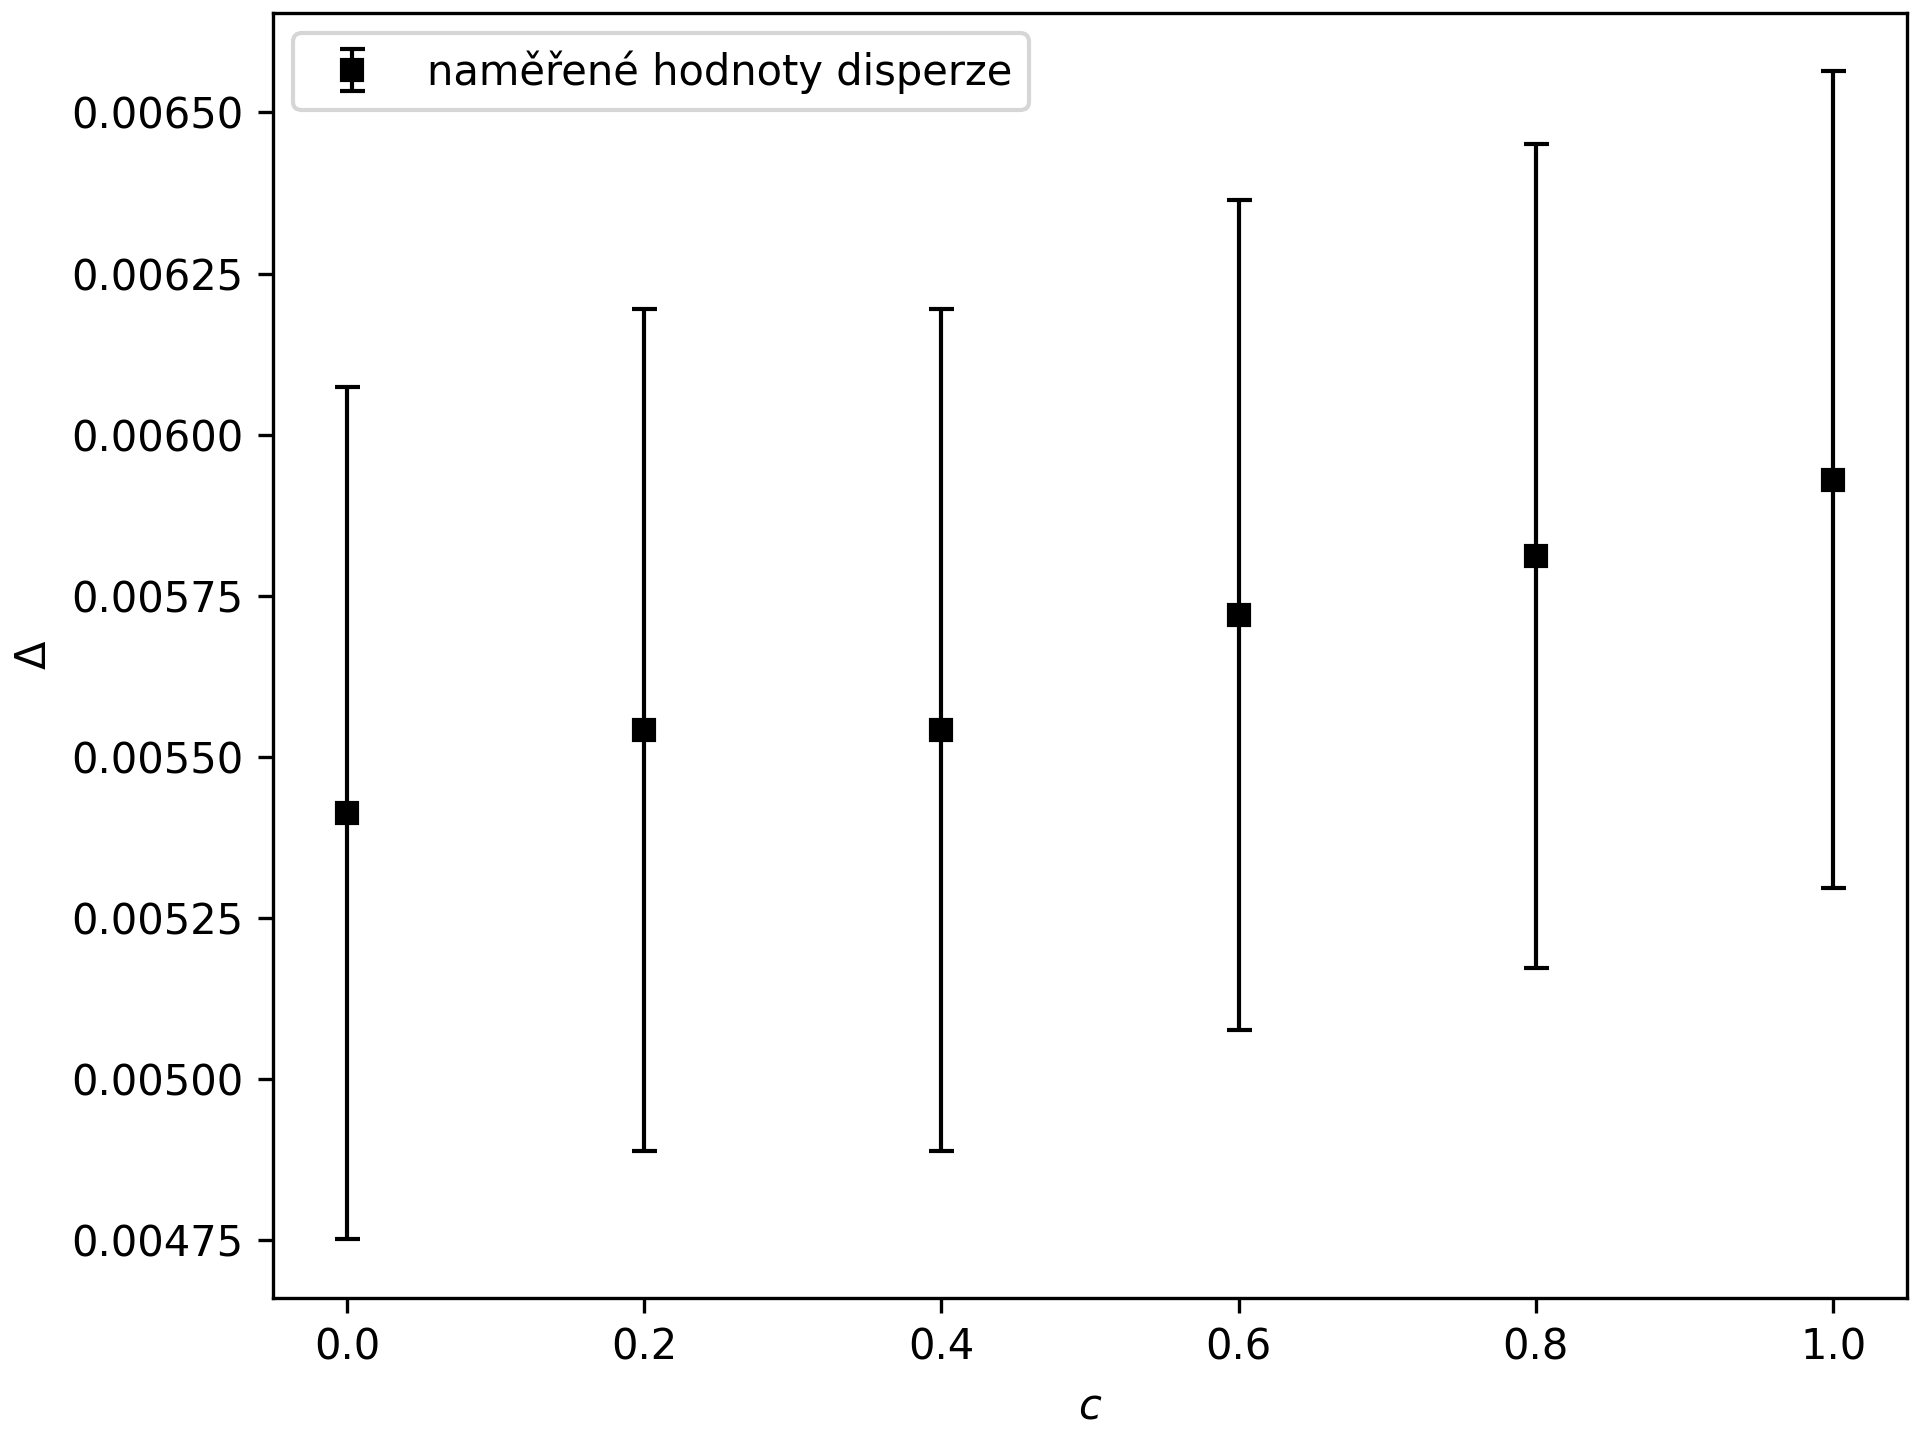
\includegraphics[width=0.5\linewidth]{glukoza_delta.png}
    \caption{Závislost střední disperze roztoku glukózy na~koncentraci vzorku.}
    \label{fig:glukoza_delta}
\end{figure}

Datovými body v~závislosti indexu lomu na~objemové koncentraci roztoku byla proložena lineární závislost
ve tvaru $N_D = a \cdot c + b$, přičemž koeficienty $a$ a~$b$ byly určeny metodou nejmenších čtverců 
pomocí funkce \texttt{curve\_fit} knihovny \texttt{scipy.optimize} jako $a = 5.53(6) \cdot 10^{-2}$,
$b = 1.3323(7)$ (nejistota byla analogicky jako v~(\ref{eq:glukoza_sigma_n}) upravena o~nejistotu indexu lomu
$\sigma_{\overline{N}_D}$).

% ================================== asi hotovo
\subsection{Index lomu polokoule}

Před měření indexů lomu vzorků optických skel bylo potřeba určit index lomu (případně sinus mezního úhlu 
$\alpha_{m0})$ skleněné polokoule. Mezní úhel pro~samotnou polokouli ve~vzduchu ($N_2 = 1)$ byl
proměřován pro~různé úhly natočení polokoule okolo svislé osy $\varphi$ s~krokem $30 \,\degree$. Pro~úhel
$\varphi = 0 \,\degree$ bylo provedeno více měření, z~nichž byla odhadnuta nejistota určení mezního úhlu.
Naměřené hodnoty jsou v~tabulce \ref{tab:mezni_phi0}. Nejistota byla vypočtena podle \cite{englich} 
(zde je nutné uvažovat směrodatnou odchylku jednoho měření, ne směrodatnou odchylku aritmetického průměru) jako
\begin{equation}
    \label{eq:sigma_alpha}
    \sigma_\alpha = \sqrt{\sigma_{\alpha,A}^2 + \sigma_{\alpha,B}^2} =
    \sqrt{ \frac{\sum_{i=1}^{5} (\alpha_{m0,i} - \overline{\alpha}_{m0})^2 }{4} + \sigma_{\alpha,B}^2} 
    = 0.02 \,\degree \,,
\end{equation}
kde $\overline{\alpha}_{m0}$ průměr naměřených hodnot mezního úhlu pro~$\varphi = 0\,\degree$ 
a~$\sigma_{\alpha,B} = 1'$ je nejistota odečtení pozice dalekohledu na~stupnici.

\begin{table}[!htbp]
\centering
\caption{Mezní úhly polokoule ve~vzduchu pro~stanovení nejistoty mezního úhlu}
\begin{tabular}{cc}
 \toprule
 číslo měření & $\alpha_{m0}\, (\mathrm{\degree})$ \\
 \midrule
 $1$ & $34.950$ \\
 $2$ & $34.967$ \\
 $3$ & $34.950$ \\
 $4$ & $34.983$ \\
 $5$ & $34.983$ \\
 \midrule
 průměr & $34.97(2)$ \\
 \bottomrule
\end{tabular}
\label{tab:mezni_phi0}
\end{table}

Z~mezních úhlů byl podle vztahu (\ref{eq:mezni}) s~$N_2 = 1$ vypočten odpovídající index lomu skleněné polokoule.
Nejistota indexu lomu je podle \cite{englich} daná vztahem
\begin{equation}
    \label{eq:sigma_N1}
    \sigma_{N_1} = N_1 \tan \alpha_{m0} \sigma_\alpha \,.
\end{equation}
Mezní úhly a~indexy lomu polokoule ve~vzduchu pro~různé úhly otočení okolo svislé osy jsou v~tabulce
\ref{tab:polokoule}. Mezní úhel měnící se~s~otočením je navíc vykreslen na~obrázku \ref{fig:mezni_polokoule}.
Za~předpokladu, že index lomu materiálu polokoule nezávisí na~směru šíření paprsku, je zřejmé, že polokoule nebyla v~držáku
umístěna dokonale vodorovně, ale byla lehce ukloněná o~úhel $\delta$. Z~fitu pomocí funkce \texttt{curve\_fit} sinovou
závislostí ve~tvaru
\begin{equation}
    \label{eq:sinovy_fit}
    \alpha_{m0} = \overline{\alpha}_{m0} + \delta \sin \left(\varphi - \varphi_0\right) \,
\end{equation}
byl určen střední mezní úhel $\overline{\alpha}_{m0} = 34.88(2)\,\degree$ (nejistota získaná z~fitu byla
ještě upravena o~nejistotu určení úhlu $\sigma_\alpha$ získanou z~rovnice (\ref{eq:sigma_alpha})). 
Ze~středního mezního úhlu pak podle rovnice (\ref{eq:mezni})
vychází střední index lomu polokoule jako $\overline{N}_1 = 1.7489(10)$, přičemž nejistota byla vypočtena
analogicky jako v~(\ref{eq:sigma_N1}). Polokoule je vůči svislému směru ukloněna o~úhel $\delta = 0.26(2)\,\degree$,
proto bude v~dalších úkolech potřeba provést různé korekce.


% Z~indexů lomu byl následně vypočítán průměr $\overline{N}_1 = 1.749(5)$, přičemž 
% jeho nejistota byla vypočtena podle \cite{englich} jako (zde již opět počítám směrodatnou odchylku
% aritmetického průměru):
% \begin{equation}
%     \label{eq:sigma_bar_N1}
%     \sigma_{\overline{N}_1} = \sqrt{ \frac{\sum_{i=1}^{12} (N_{1,i} - \overline{N}_1)^2 }{11\cdot 12}} \,,
% \end{equation}
% jelikož nejistota jednotlivých indexů lomu (vypočtená podle (\ref{eq:sigma_N1})) je zanedbatelná vůči 
% statistické nejistotě (dané rozptylem indexů lomu pro~různé hodnoty $\varphi$).

\begin{table}[!htbp]
\centering
\caption{Mezní úhly a~indexy lomu polokoule ve~vzduchu v~závislosti na~otočení okolo svislé osy.}
\begin{tabular}{cccc}
 \toprule
 $\varphi\, (\mathrm{\degree})$ & $\alpha_{m0}\, (\mathrm{\degree})$ & $\sin{\alpha_{m0}}$ & $N_1$ \\
 \midrule
 $0(2)$ & $34.97(2)$ & $0.5731(3)$ & $1.745(1)$ \\
 $30(2)$ & $35.08(2)$ & $0.5748(3)$ & $1.740(1)$ \\
 $60(2)$ & $35.13(2)$ & $0.5755(3)$ & $1.738(1)$ \\
 $90(2)$ & $35.12(2)$ & $0.5752(3)$ & $1.738(1)$ \\
 $120(2)$ & $35.07(2)$ & $0.5745(3)$ & $1.741(1)$ \\
 $150(2)$ & $34.87(2)$ & $0.5717(3)$ & $1.749(1)$ \\
 $180(2)$ & $34.75(2)$ & $0.5700(3)$ & $1.754(1)$ \\
 $210(2)$ & $34.67(2)$ & $0.5688(3)$ & $1.758(1)$ \\
 $240(2)$ & $34.65(2)$ & $0.5686(3)$ & $1.759(1)$ \\
 $270(2)$ & $34.65(2)$ & $0.5686(3)$ & $1.759(1)$ \\
 $300(2)$ & $34.72(2)$ & $0.5695(3)$ & $1.756(1)$ \\
 $330(2)$ & $34.83(2)$ & $0.5712(3)$ & $1.751(1)$ \\
 \bottomrule
\end{tabular}
\label{tab:polokoule}
\end{table}


\begin{figure}
    \centering
    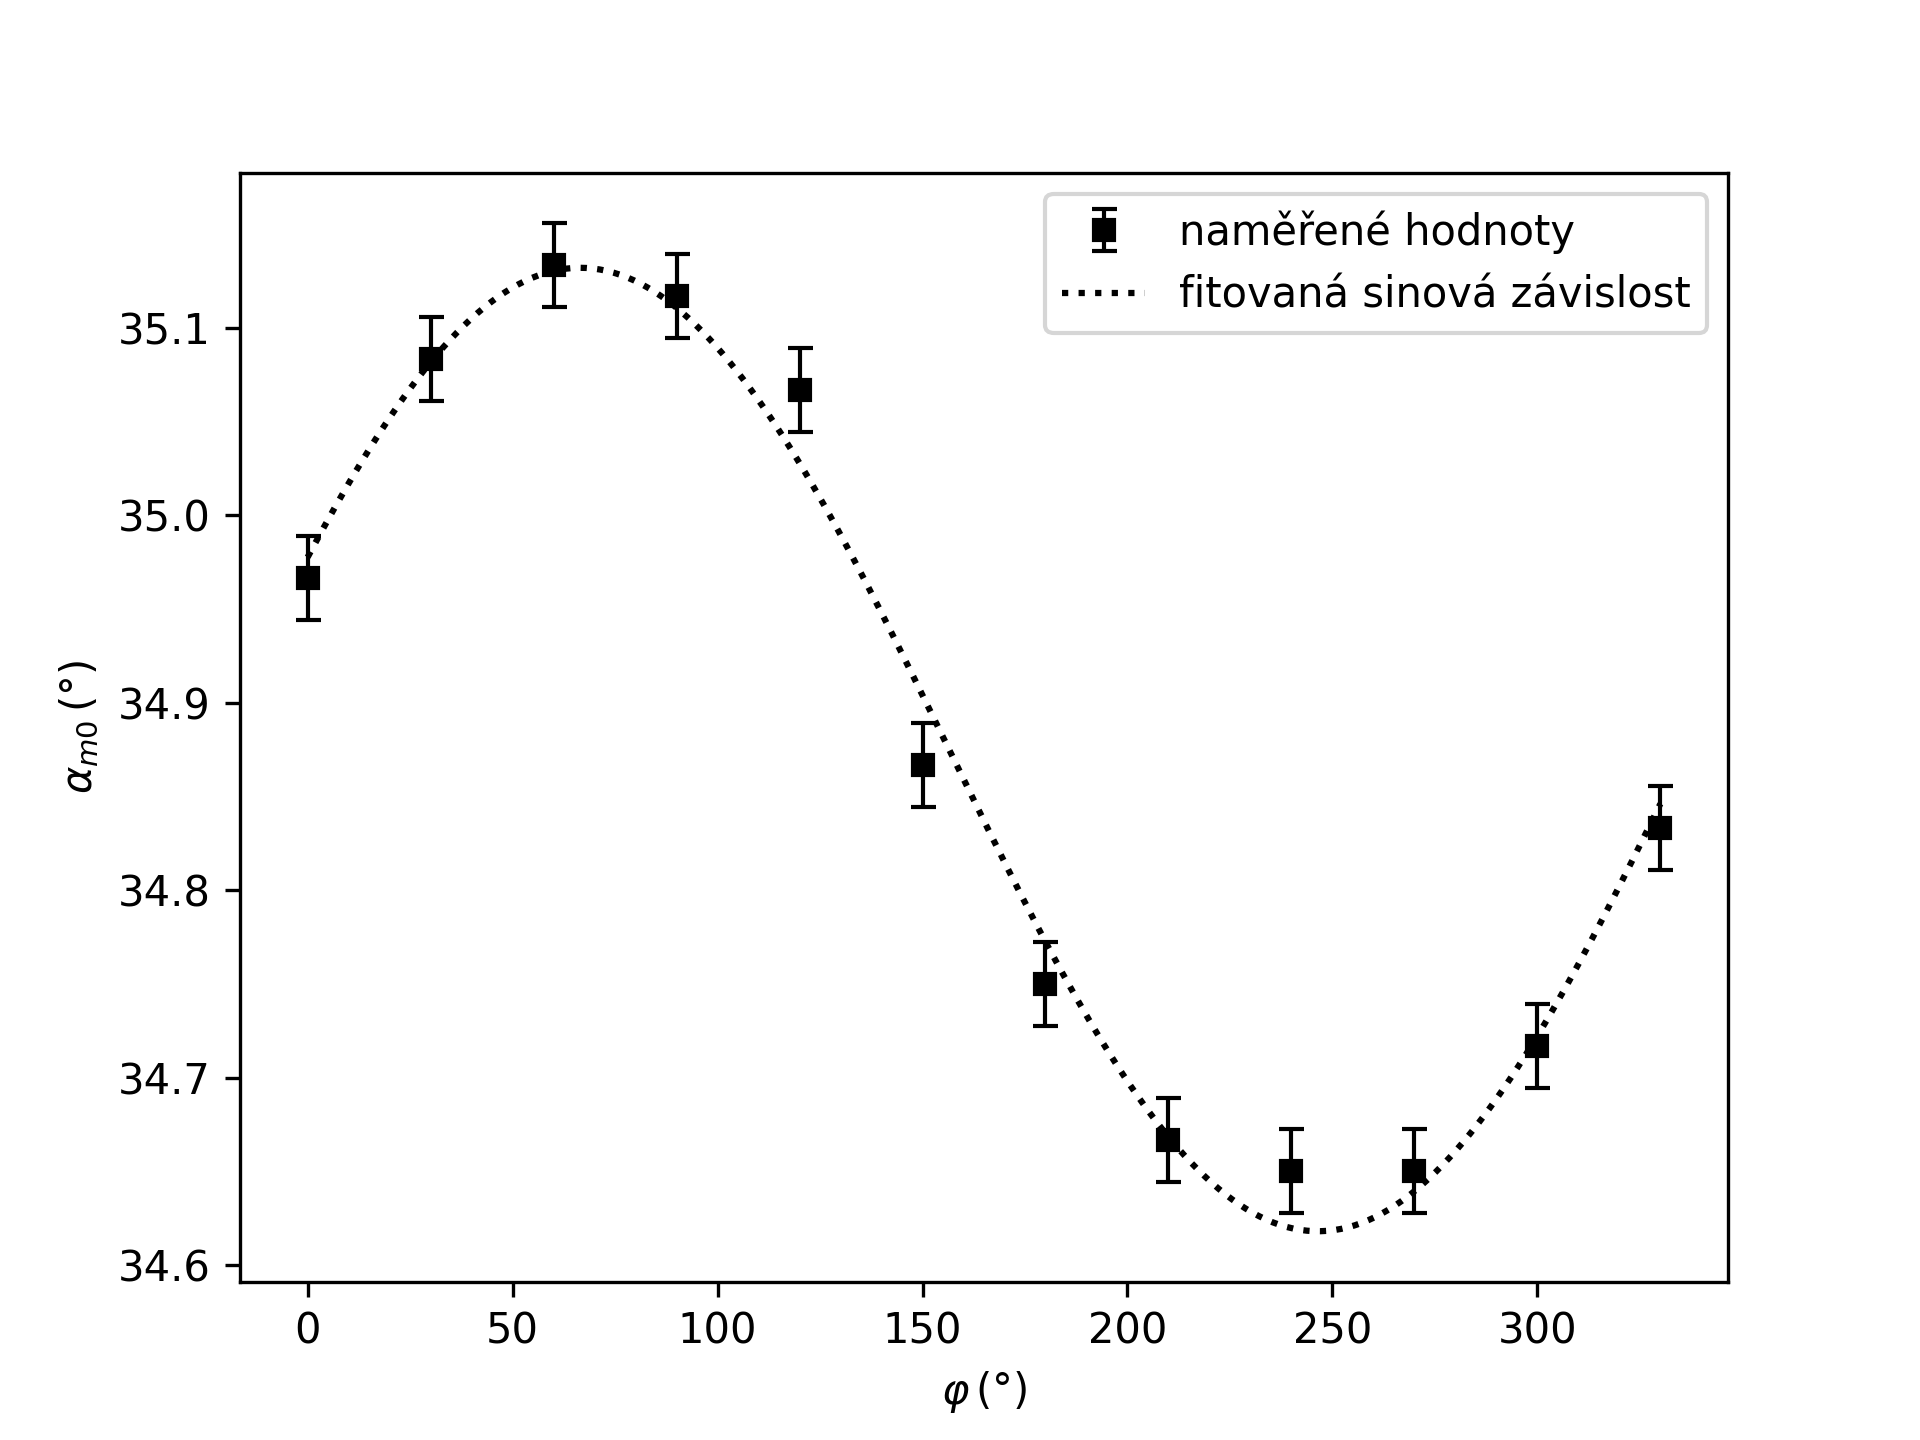
\includegraphics[width=0.6\linewidth]{polokoule.png}
    \caption{Závislost mezního úhlu polokoule na úhlu otočení kolem svislé osy. Horizontální chybové úsečky
    nebyly pro~svou malou velikost pro~přehlednost vykresleny.}
    \label{fig:mezni_polokoule}
\end{figure}

% ==================================
\subsection{Index lomu vzorků optických skel}

Následně byly na~vrchní stěnu polokoule pokládány vzorky optických skel a~opět měřeny mezní úhly. Proměřován
byl vzorek o~známém indexu lomu $N_{znamy,tab}=1.5160$, simax a optické sklo číslo 3. Kvůli nevodorovnému umístění
polokoule v~držáku byly změřeny dva mezní úhly, jeden pro~$\varphi = 0\,\degree$ a~druhý pro~$\varphi = 180\,\degree$,
z~nichž byl vypočten průměr. Odchylky od~skutečného mezního úhlu mají na~opačných stranách opačné znamínko a~vyruší
se.~Nejistota tohoto průměru byla určena podle \cite{englich} jako
\begin{equation}
    \label{eq:sigma_alpha_vzorky}
    \sigma_{\overline{\alpha}_m} = \frac{\sqrt{2}}{2} \sigma_\alpha \,.
\end{equation}

Z~mezních úhlů byly podle vztahu (\ref{eq:indexvzorku}) vypočteny indexy lomu vzorků (jsou uvedeny 
v~tabulce \ref{tab:vzorky}), přičemž jejich nejistota je dána jako \cite{englich}
\begin{equation}
    \label{eq:sigma_index_vzorku}
    \sigma_{N_2} = N_2 \sqrt{ \relsqr{\overline{N}_1} + \left(\frac{\sigma_{\overline{\alpha}_m}} 
    {\tan \overline{\alpha}_m}\right)^2 } \,.
\end{equation}

\begin{table}[!htbp]
\centering
\caption{Mezní úhly a indexy lomu vzorků optických skel}
\begin{tabular}{ccccc}
 \toprule
 vzorek & $\alpha_1\, (\degree)$ & $\alpha_2\, (\degree)$ & $\overline{\alpha}_m\, (\degree)$ & $N_2$\\
 \midrule
 sklo s $N_2=1.5160$ & $60.32(2)$ & $59.87(2)$ & $60.092(16)$ & $1.5160(9)$ \\
 simax & $57.90(2)$ & $57.23(2)$ & $57.567(16)$ & $1.4761(9)$ \\
 optické sklo č. 3 & $65.10(2)$ & $64.40(2)$ & $64.750(16)$ & $1.5818(9)$ \\
 \bottomrule
\end{tabular}
\label{tab:vzorky}
\end{table}


% ==================================
\subsection{Index lomu křemene}

Nakonec byl na~vrchní stěnu polokoule umístěn vzorek křemene a~pro~různé úhly natočení polokoule
byly měřeny mezní úhly řádného a~mimořádného paprsku. Z~rovnice (\ref{eq:indexvzorku}) byly vypočteny
jejich indexy lomu, přičemž nejistota byla určena podle vztahu (\ref{eq:sigma_index_vzorku}). 
Naměřené hodnoty jsou uvedeny v~tabulce \ref{tab:kremen_uhly} a~vykresleny v~grafu \ref{fig:kremen_raw}.


\begin{table}[!htbp]
\centering
\caption{Mezní úhel a index lomu řádného a mimořádného paprsku křemene v~závislosti na~natočení polokoule
kolem svislé osy.}
\begin{tabular}{ccccc}
 \toprule
  & \multicolumn{2}{c}{řádný paprsek} & \multicolumn{2}{c}{mimořádný paprsek} \\
 $\varphi\, (\mathrm{\degree})$ & $\alpha_o\, (\mathrm{\degree})$ & $N_o$ & $\alpha_e\, (\mathrm{\degree})$ & $N_e$ \\
 \midrule
 $0(2)$ & $62.25(2)$ & $1.548(1)$ & $62.27(2)$ & $1.548(1)$ \\
 $30(2)$ & $62.32(2)$ & $1.549(1)$ & $62.35(2)$ & $1.549(1)$ \\
 $60(2)$ & $62.32(2)$ & $1.549(1)$ & $62.65(2)$ & $1.553(1)$ \\
 $90(2)$ & $62.05(2)$ & $1.545(1)$ & $62.65(2)$ & $1.553(1)$ \\
 $120(2)$ & $61.95(2)$ & $1.543(1)$ & $62.50(2)$ & $1.551(1)$ \\
 $150(2)$ & $61.77(2)$ & $1.541(1)$ & $62.07(2)$ & $1.545(1)$ \\
 $180(2)$ & $61.55(2)$ & $1.538(1)$ & $61.58(2)$ & $1.538(1)$ \\
 $210(2)$ & $61.58(2)$ & $1.538(1)$ & $61.62(2)$ & $1.539(1)$ \\
 $240(2)$ & $61.60(2)$ & $1.538(1)$ & $61.97(2)$ & $1.544(1)$ \\
 $270(2)$ & $61.82(2)$ & $1.542(1)$ & $62.43(2)$ & $1.550(1)$ \\
 $300(2)$ & $61.95(2)$ & $1.543(1)$ & $62.50(2)$ & $1.551(1)$ \\
 $330(2)$ & $62.10(2)$ & $1.546(1)$ & $62.43(2)$ & $1.550(1)$ \\
 \bottomrule
\end{tabular}
\label{tab:kremen_uhly}
\end{table}

\begin{figure}[!htbp]
    \centering
    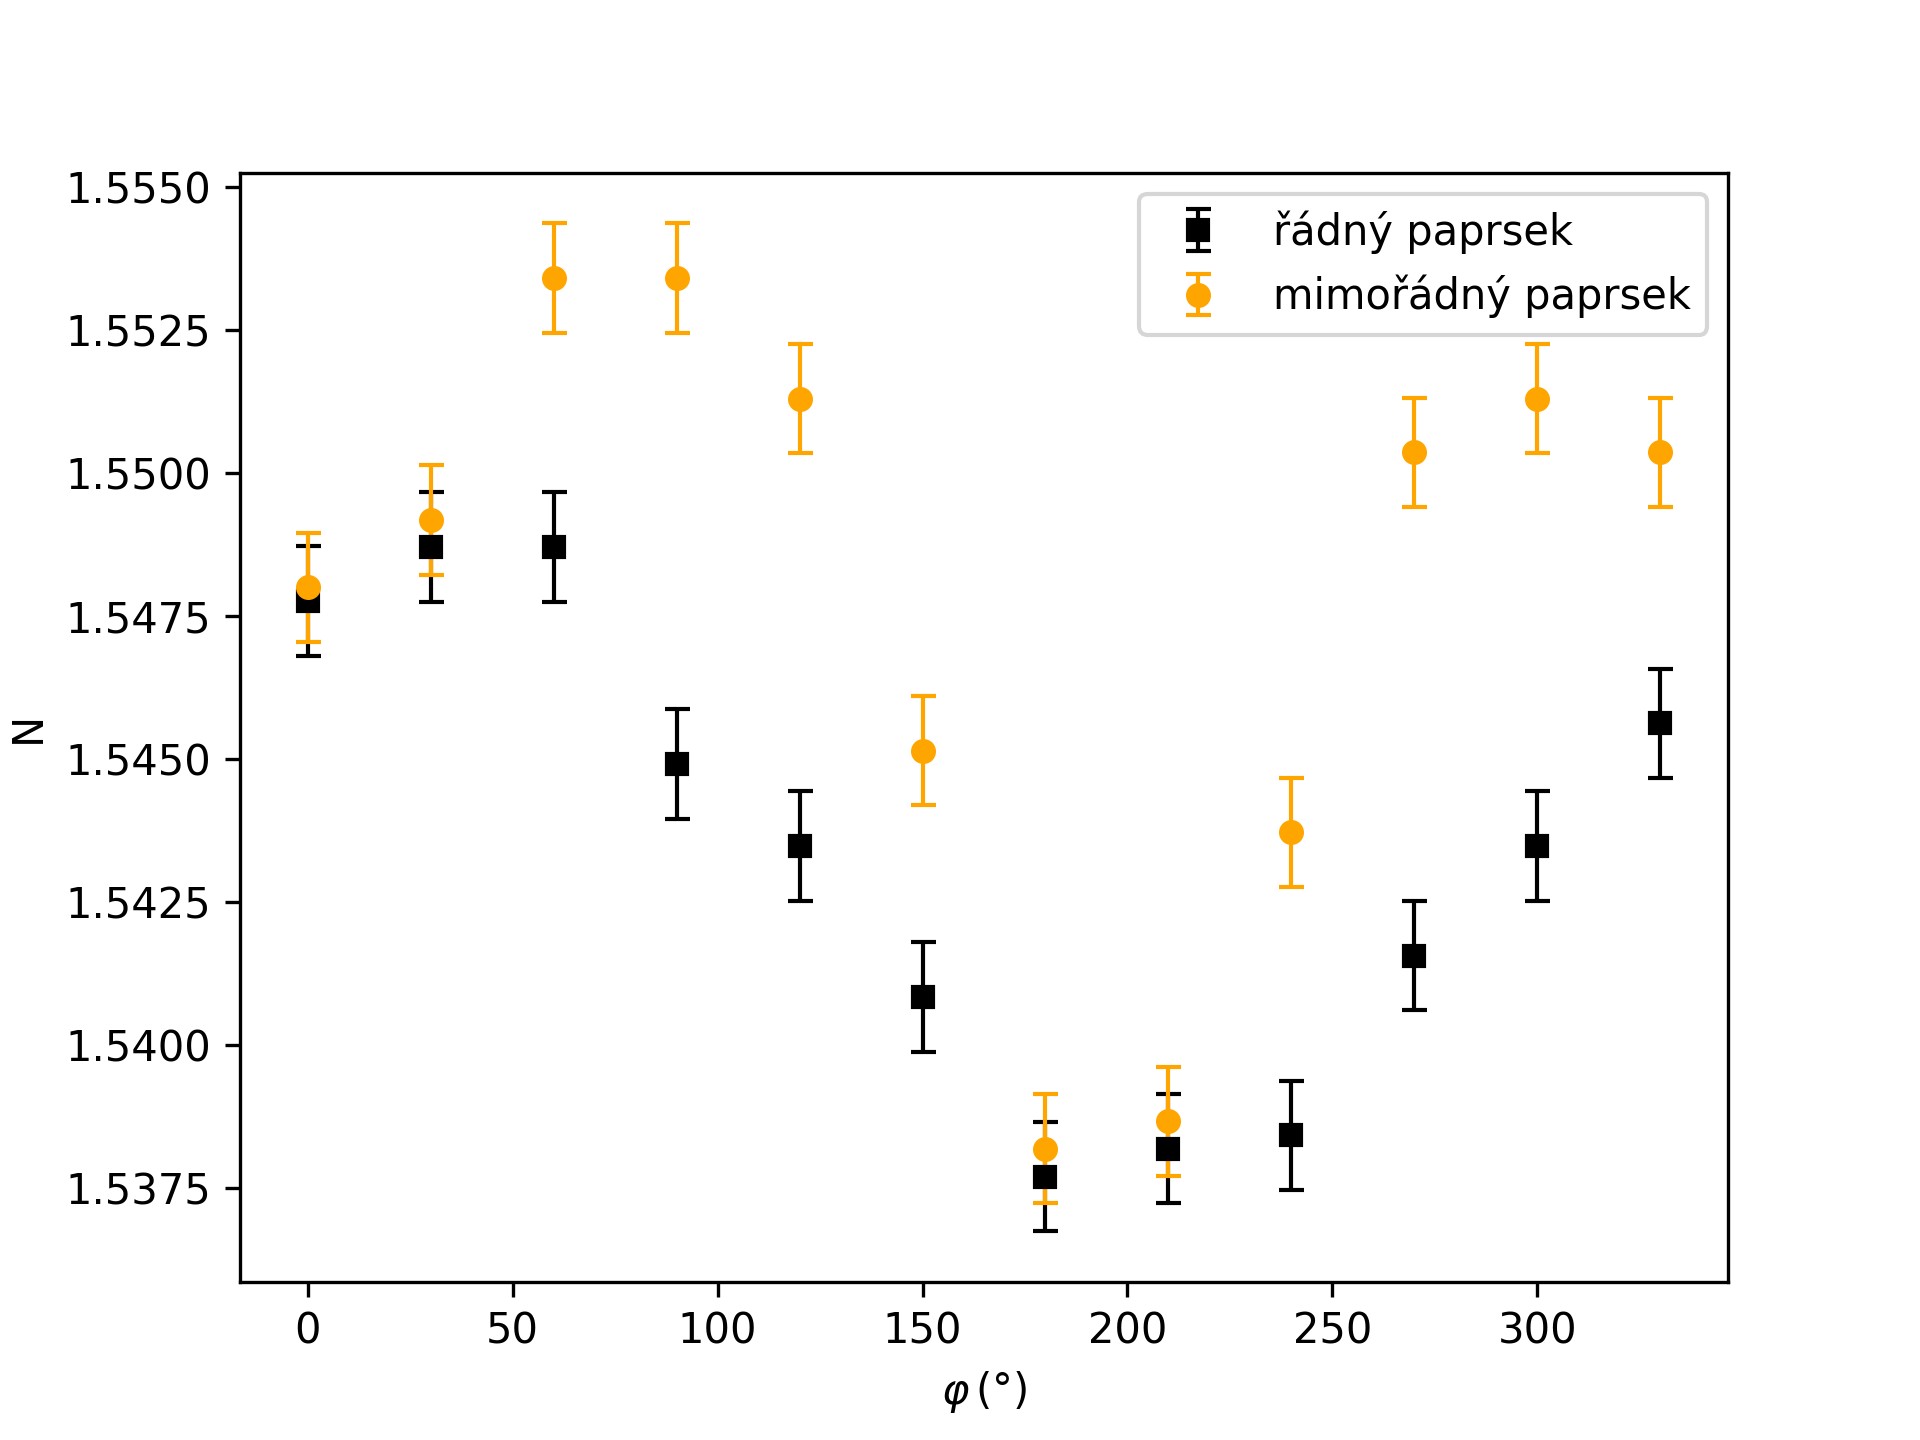
\includegraphics[width=0.6\linewidth]{kremen_raw.png}
    \caption{Závislost indexu lomu řádného a mimořádného paprsku ve vzorku křemene na~úhlu natočení 
    polokoule~-~bez korekce. Horizontální chybové úsečky nebyly pro~svou malou velikost pro~přehlednost vykresleny.}
    \label{fig:kremen_raw}
\end{figure}

Z~grafu \ref{fig:kremen_raw} je zřejmé, že je potřeba provést korekci na~nedokonalé umístění polokoule
v~držáku. Střední mezní úhel řádného paprsku byl určen analogickým způsobem jako při~měření indexu lomu
sklěněné polokoule - z~fitu sinovou závislostí (k~nahlédnutí v~grafu \ref{fig:kremen_raw_angles}) byla získána
hodnota $\overline{\alpha}_o = 61.94(2)$, odkud $\overline{N}_o = 1.543(1)$. S~ohledem na~předpoklad, že~index 
lomu řádného paprsku nezávisí na~směru šíření, byla provedena korekce mezních úhlů mimořádného paprsku
podle vzorce:
\begin{equation}
    \label{eq:correction}
    \alpha_{e,i} = \alpha_{e,i}' - \left(\alpha_{o,i}' - \overline{\alpha}_o\right) \,,
\end{equation}
kde $i$ je~index odpovídající určitému úhlu natočení polokoule, $\alpha_{e,i}'$ a~$\alpha_{o,i}'$ 
jsou~naměřené mezní úhly mimořádného a~řádného paprsku. Korigované hodnoty mezních úhlů a~odpovídající
indexy lomu jsou uvedeny v~tabulce \ref{tab:kremen_correction} a~vykresleny v~grafu \ref{fig:kremen_corrected}.

\begin{figure}[!htbp]
    \centering
    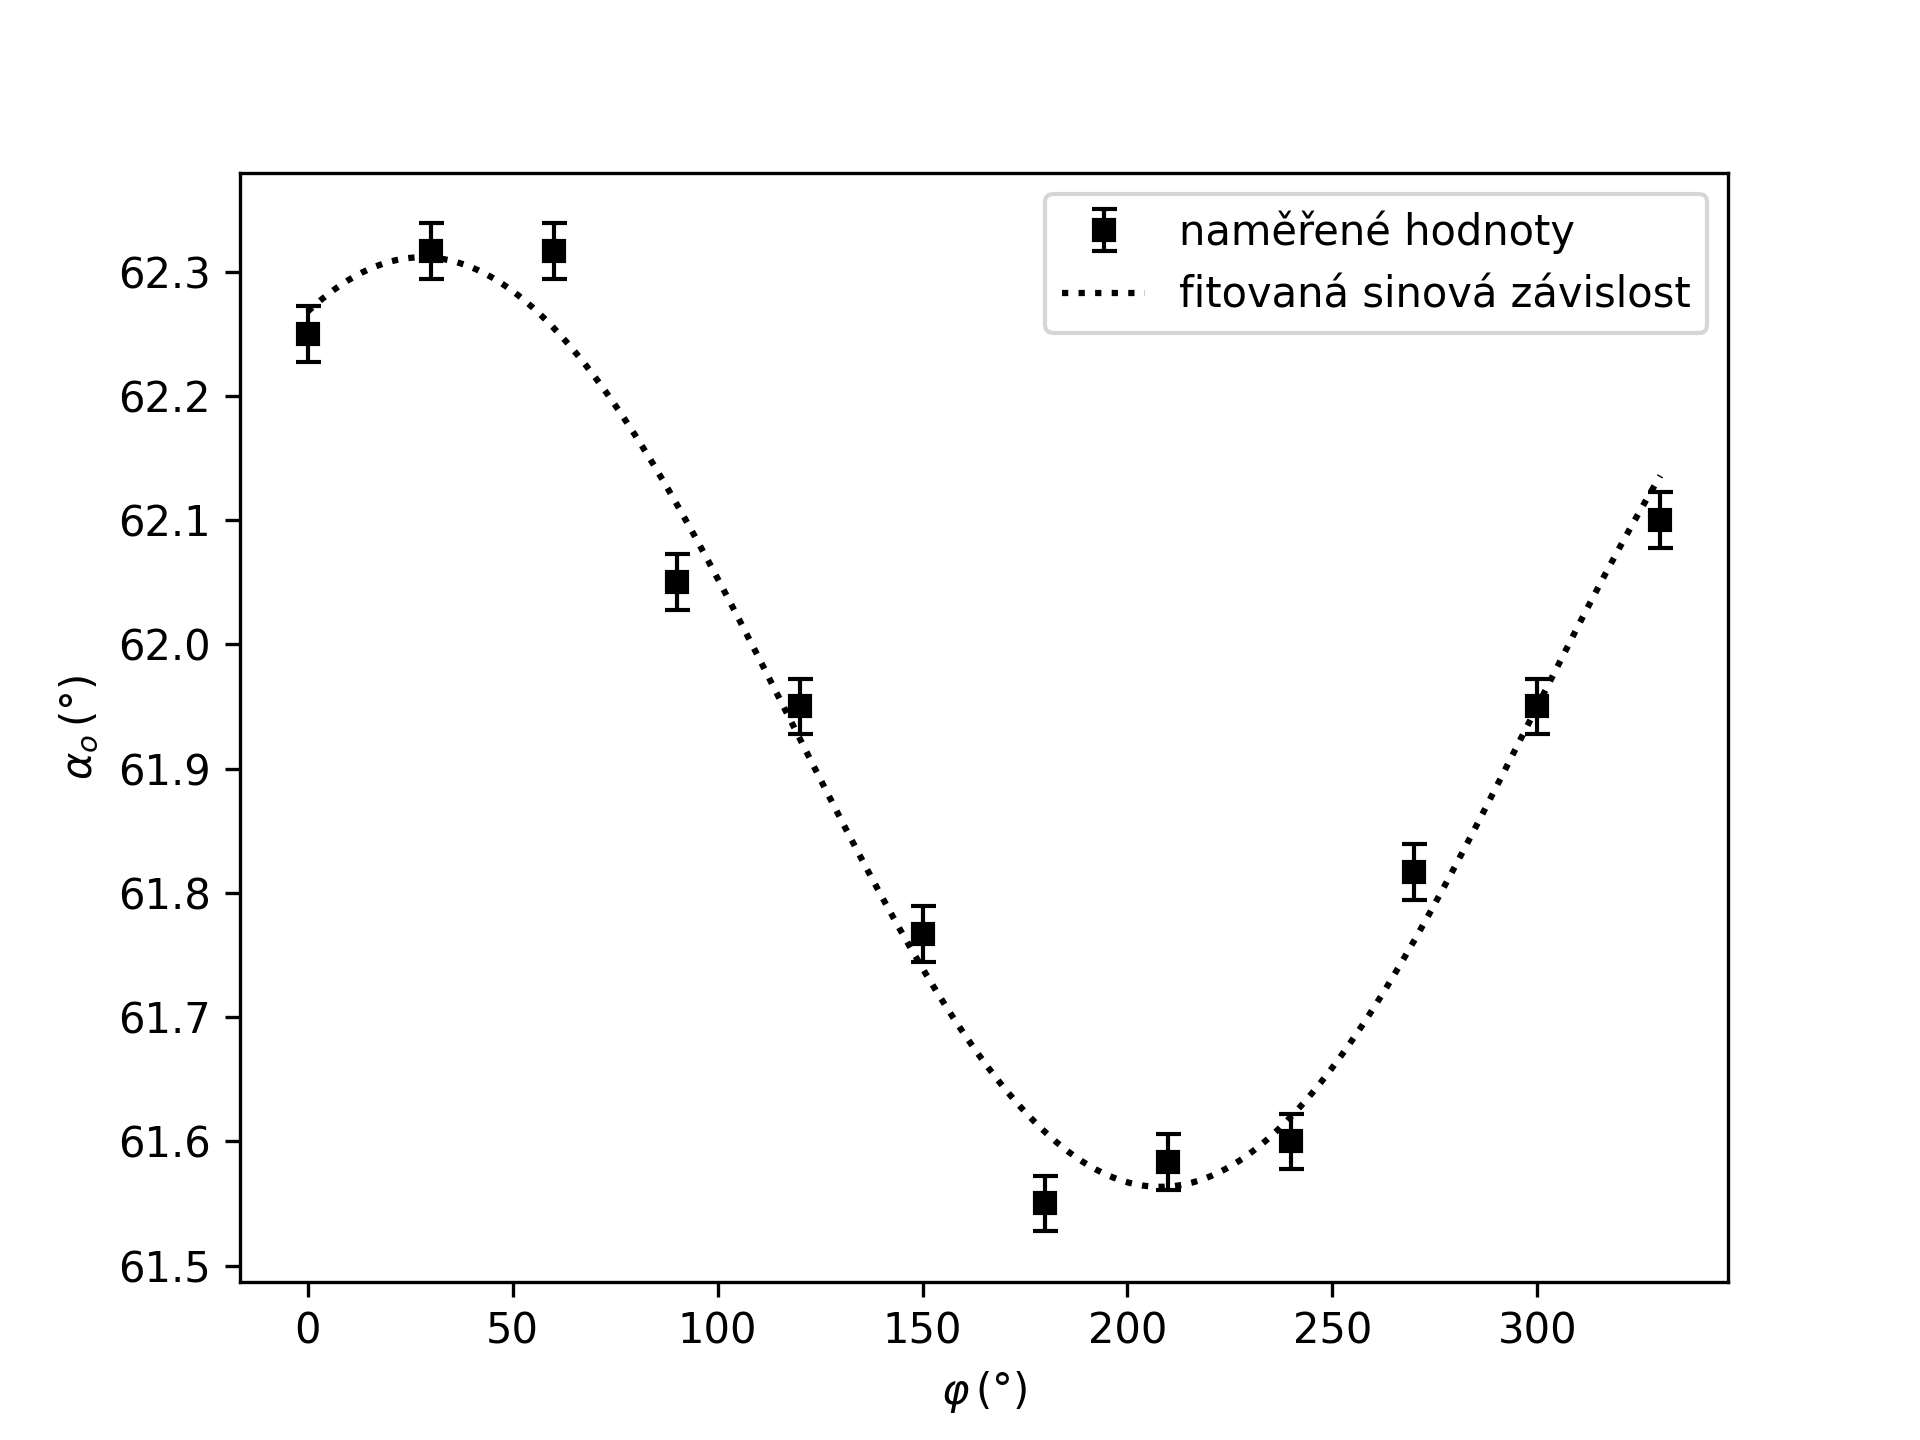
\includegraphics[width=0.6\linewidth]{kremen_raw_angles.png}
    \caption{Závislost mezního úhlu řádného paprsku ve vzorku křemene na~úhlu natočení polokoule. 
    Horizontální chybové úsečky nebyly pro~svou malou velikost pro~přehlednost vykresleny.}
    \label{fig:kremen_raw_angles}
\end{figure}

\begin{table}[!htbp]
\centering
\caption{Mezní úhly a indexy lomu mimořádného paprsku ve vzorku křemene v~závislosti na~natočení polokoule
- po~korekci.}
\begin{tabular}{ccc}
 \toprule
 $\varphi\, (\mathrm{\degree})$ & $\alpha_e\, (\mathrm{\degree})$ & $N_e$ \\
 \midrule
 $0(2)$ & $61.95(4)$ & $1.5435(11)$ \\
 $30(2)$ & $61.97(4)$ & $1.5438(11)$ \\
 $60(2)$ & $62.27(4)$ & $1.5481(11)$ \\
 $90(2)$ & $62.54(4)$ & $1.5518(11)$ \\
 $120(2)$ & $62.49(4)$ & $1.5511(11)$ \\
 $150(2)$ & $62.24(4)$ & $1.5476(11)$ \\
 $180(2)$ & $61.97(4)$ & $1.5438(11)$ \\
 $210(2)$ & $61.97(4)$ & $1.5438(11)$ \\
 $240(2)$ & $62.30(4)$ & $1.5485(11)$ \\
 $270(2)$ & $62.55(4)$ & $1.5521(11)$ \\
 $300(2)$ & $62.49(4)$ & $1.5511(11)$ \\
 $330(2)$ & $62.27(4)$ & $1.5481(11)$ \\
 \bottomrule
\end{tabular}
\label{tab:kremen_correction}
\end{table}

\begin{figure}[!htbp]
    \centering
    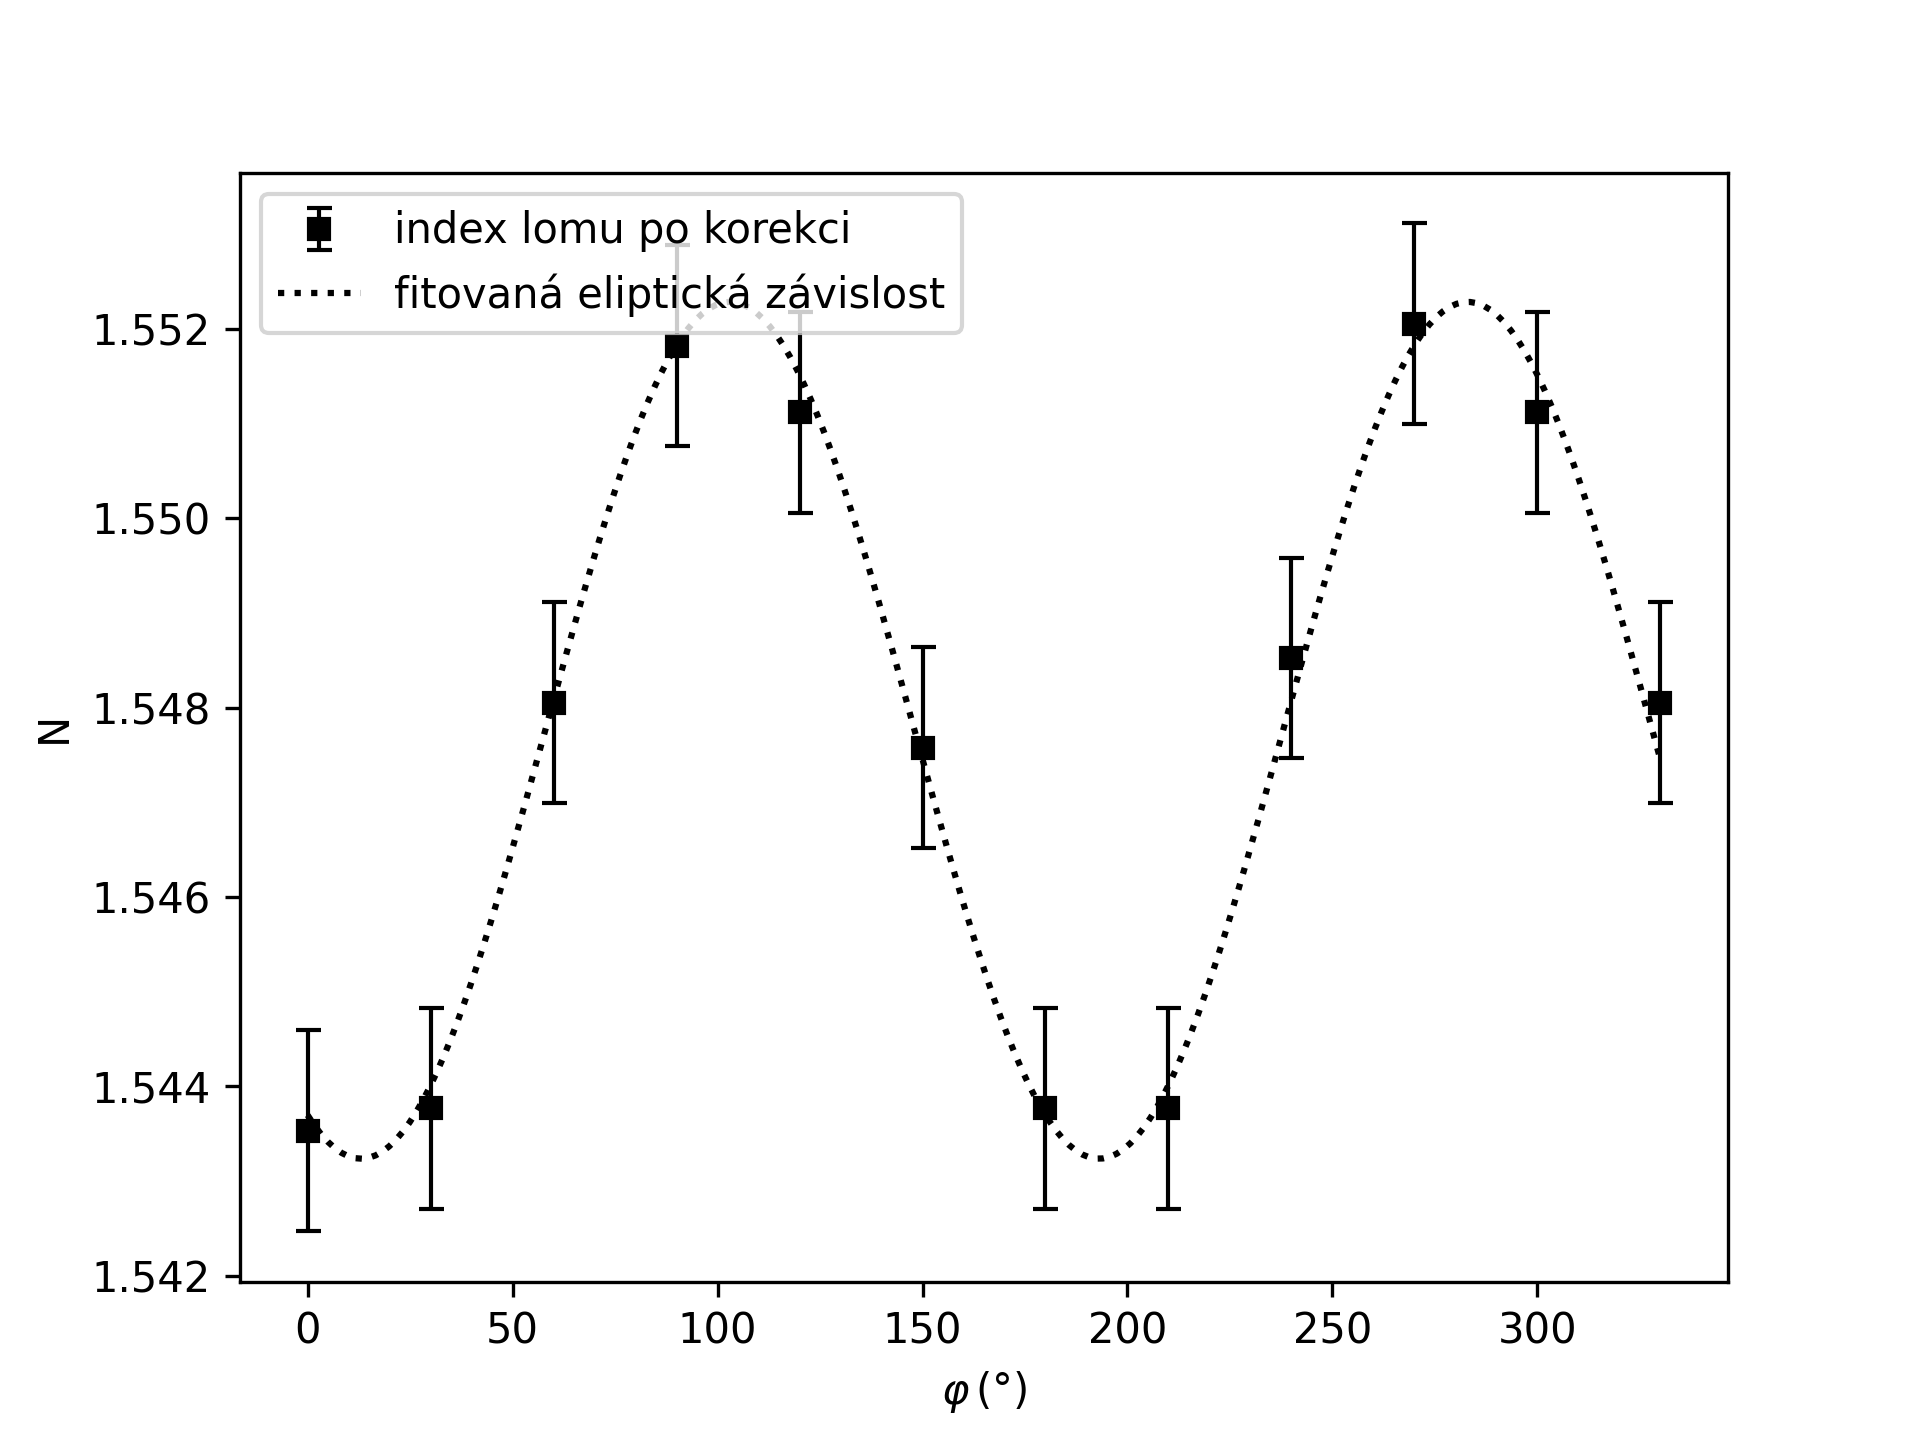
\includegraphics[width=0.6\linewidth]{kremen_corrected.png}
    \caption{Závislost indexu lomu mimořádného paprsku ve vzorku křemene na~úhlu natočení
    polokoule ~-~po~korekci. Horizontální chybové úsečky nebyly pro~svou malou 
    velikost pro~přehlednost vykresleny.}
    \label{fig:kremen_corrected}
\end{figure}

Datovými body v~grafu \ref{fig:kremen_corrected} byla proložena závislost ve~tvaru
\begin{equation}
    \label{eq:elliptic_fit}
    N_e = \sqrt{ N_{o,D}^2 \cos^2 \left( \varphi - \varphi_0 \right) +
    N_{e,D}^2 \sin^2 \left( \varphi - \varphi_0 \right)} \,,
\end{equation}
popisující vzdálenost bodu na~elipse (na~řezu indexového elipsoidu) od~středu elipsy, tedy velikost indexu lomu
mimořádného paprsku v~závislosti na~směru šíření $\varphi$ (odvozeno podle teorie v~\cite{franc}). $N_{o,D}$
a~$N_{e,D}$ jsou hlavní řádný resp. mimořádný index lomu křemene pro~spektrální čáru D
($\lambda_\mathrm{Na} = \qty{589.3}{nm}$).

Z~fitu pomocí funkce \texttt{curve\_fit} vycházejí koeficienty $N_{o,D} = 1.5432(10)$ a~$N_{e,D} = 1.5523(10)$
(nejistoty byly upraveny o~nejistotu určení indexu lomu podle \ref{eq:sigma_index_vzorku}). Jedná se~tedy 
o~kladný jednoosý krystal.

% ============================ DISKUZE ===============================
\section{Diskuze}

Všechny indexy lomu naměřené během úhlohy odpovídají spektrální čáře D sodíkového dubletu 
($\lambda_\mathrm{Na}=\qty{589.3}{nm}$). Dvouhranolový refraktometr využíval dvojici Amiciho hranolů, kde
každý z~nich byl vyroben tak, aby jimi právě spektrální čára D prošla beze změny směru. Ostatní složky bílého světla
pak byly natočením dvojice hranolů vůči sobě srovnány tak, aby se~šířily ve~stejném směru jako paprsek D
a~kompenzovala se~tak disperze od~vzorku, jež by v~refraktometru způsobila neostré a~barevné rozhranní světlo-stín.
Při~měření s~polokulovým refraktometrem pak byla přímo použita sodíková výbojka s~maximem intenzity
na~této vlnové délce.

% =================== hotovo
\textit{Index lomu a střední disperze roztoku glukózy.} Absolutní koeficient $b=1.3323(7)$ (relativní nejistota
$0.05\,\%$) odpovídá indexu lomu
roztoku o~nulové koncentraci, tedy indexu lomu destilované vody. Tabulková hodnota je $N_{D,dest,tab} = 1.333$ 
\cite{mikulcak}, což v~rámci nejistoty měření odpovídá experimentální hodnotě. Pro~$100\%$ roztok
je index lomu $N_{D,gluk} = 1.3887(5)$ (rel. nej. $0.05\,\%$). Hodnoty indexu lomu se~daly určit velmi přesně
díky velké přesnosti stupnice v~refraktometru. Závislost indexu lomu na~koncentraci roztoku lze poměrně přesně
popsat lineární funkcí, jak ukazuje graf \ref{fig:glukoza_n}. 

Střední disperze $0\%$ roztoku
vychází $\Delta_{dest} = 0.0054(7)$ s~relativní nejistotou $13\,\%$, přičemž tabulková hodnota je 
$\Delta_{dest,tab} = 0.006$ \cite{mikulcak}, což v~rámci nejistoty měření odpovídá experimentální hodnotě.
Pro~$100\%$ koncentraci pak byla naměřena $\Delta_{gluk} = 0.0059(6)$ (rel. nej. $10\,\%$). 
Velká nejistota disperze je dána především nejistotou parametru $\sigma$, který je jednoznačně určen pozicí 
Amiciho hranolů vůči sobě. Kvůli velké nejistotě stupnice $Z$ se~nedal určit s~větší přesností.
Datovými body střední disperze nebyla
proložena lineární závislost, neboť dispeze není jednoduchou lineární funkcí koncentrace roztoku. I~když 
v~rámci nejistoty měření ji lze lineární funkcí aproximovat.

Index lomu i~střední disperze budou silně záviset na~teplotě roztoku, proto byla během měření s~pomocí přiloženého
digitálního teploměru zaznamenávána teplota okolí. Během měření došlo k~mírnému nárůstu teploty, pravděpodobně
kvůli zdroji bílého světla, jež refraktometr kromě osvětlení i~zahříval. Tím mohly být systematicky ovlivněny
výsledky experimentu. Další nepřesnost mohla vzniknout přímo při~přípravě roztoků různých koncentrací kvůli 
nejistotě pipetovaného objemu.

% =================== hotovo
\textit{Index lomu polokoule.} Kvůli nedokonalému uložení polokoule v~držáku nevychází index lomu použitého
skla (daný mezním úhlem) konstantní, ale mění se~s~různými natočením polokoule kolem svislé osy. Koule tedy
byla pravděpodobně mírně vychýlena. Střední hodnota proto byla získána proložením datových bodů sinovou 
závislostí (\ref{eq:sinovy_fit}).
Tato metoda je přesnější než prosté vypočtení aritmetického průměru, protože rozdělení
hodnot okolo jejich střední hodnoty zřejmě není náhodné, ale lze poměrně dobře (jak je vidět z~grafu 
\ref{fig:mezni_polokoule}) popsat právě sinovou závislostí okolo střední hodnoty. Index lomu polokoule (odpovídající
střední hodnotě lámavého úhlu pro~různé úhly otočení kolem svislé osy) vychází $N_1 = 1.7489(10)$ 
(rel. nej. $0.06\,\%$), což odpovídá
hrubé hodnotě 1.7-1.8 udávané v~pokynech \cite{pokyny} pro~silně lámavé flintové sklo. Index lomu polokoule bylo nutné
určit co nejpřesněji, jelikož na~něm přímo závisí měřené indexy lomu vzorků optických skel a~křemene.

(\textit{Pozn: datové body 7, 9 a~10, které odpovídají úhlům $\varphi = 180\,\degree$, $240\,\degree$ a~$270\,\degree$,
se~nacházely zřetelně mimo závislost danou ostatními body, a~to o~zhruba $0.5\,\degree$. Zřejmě během měření
došlo ke~hrubé chybě přehlédnutí o~půl stupně, nejspíše kvůli dělení nonia na~právě 30 dílků odpovídající 30
ůhlovým minutám namísto plným 60 minutám. Proto jsou tyto hodnoty v~tabulce \ref{tab:polokoule} odlišné 
od~hodnot uvedených v~záznamu měření.})

% ====================== hotovo
\textit{Index lomu vzorků optických skel.} Index lomu vzorku skla se~známou honotou $N_\mathrm{znamy} = 1.5160(9)$ 
(rel. nejistota $0.06\,\%$) odpovídá hodnotě $N_{znamy,tab} = 1.5160$ uvedené u~vzorku. Index lomu simaxu
$N_\mathrm{simax} = 1.4761(9)$ (rel. nejistota $0.06\,\%$) je o~něco větší než tabulková hodnota 
$N_{simax,tab} = 1.472$ \cite{simax}. Odhaduji,
že index lomu bude silně záviset na~konkrétním složení vzorku a~může se~tedy mírně lišit od~hodnoty udávané
výrobcem. Index lomu vzorku optického skla č. 3 byl určen jako $N_{\# \,3} = 1.5818(9)$ (rel. nejistota $0.06\,\%$).
Všechny hodnoty splňují podmínku pro~použití monobromnaftalenu jako imerzní kapaliny ($N_1 > N_i > N_2$).

% ====================
\textit{Index lomu křemene.} Stejně jako při~měření indexu lomu skleněné polokoule není mezní úhel
řádného paprsku konstantní s~úhlem natočení polokoule (jak by mělo být pro~konstantní index lomu), 
ale lze jej relativně dobře popsat sinovou závislostí (viz graf \ref{fig:kremen_raw_angles}). Protože
index lomu řádného i~mimořádného paprsku byly pro~daný úhel $\varphi$ měřeny najednou, je korekce mezních úhlů
prováděna na~základě řádného paprsku a~nikoliv na~základě měření se~skleněnou polokoulí. Během měření
se~vzorky optických skel totiž mohlo dojít k~mírnému posunutí polokoule v~držáku a~korekce by nebyla přesná.
Indexy lomu mimořádného paprsku získané z~upravených mezních úhlů lze již velmi dobře 
(viz graf \ref{fig:kremen_corrected}) popsat teoretickou závislostí (\ref{eq:elliptic_fit}), která vysvětluje
hodnotu index lomu pomocí pozice (odpovídající směru šíření) na~indexovém elipsoidu s~hlavními poloosami $N_{o,D}$
a~$N_{e,D}$. Fitem této závislosti byly experimentálně získány hodnoty hlavních indexů lomu křemene 
$N_{o,D} = 1.5432(10)$ a~$N_{e,D} = 1.5523(10)$ (rel. nej. $0.06\,\%$), které v~rámci nejistoty měrení odpovídají
tabulkovým hodnotám $N_{o,D,tab} = 1.544$ a~$N_{e,D,tab} = 1.553$ \cite{mikulcak}. $N_{e,D} > N_{o,D}$,
křemen je tedy kladný jednoosý krystal.

% ============================= ZÁVĚR ================================
\section{Závěr}

Bylo změřeno, že index lomu roztoku glukózy závisí lineárně na~jeho koncentraci s~kladným lineárním koeficientem.
Index lomu roztoku o~nulové koncentraci, tedy destilované vody vychází $N_{D,dest}=1.3323(7)$ a~pro~100\% koncentraci
$N_{D,gluk} = 1.3887(5)$. Střední disperze
glukózy roste s~koncentrací roztoku, pro nulovou koncentraci je střední disperze $\Delta = 0.0054(7)$
a~pro~100\% koncentraci $\Delta = 0.0059(6)$.

Index lomu skleněné polokoule v~polokulovém refraktometru byl určen jako $N_1 = 1.7489(10)$. Index lomu
vzorku skla se~známou hodnotou indexu lomu je $N_\mathrm{znamy} = 1.5160(9)$, index lomu simaxu je 
$N_\mathrm{simax} = 1.4761(9)$ a~index lomu vzorku optického skla č. 3 byl určen jako $N_\mathrm{\# \,3} = 1.5818(9)$.


Index lomu řádného paprsku křemene byl stanoven jako $N_{o,D} = 1.5432(10)$ a~pro~mimořádný paprsek vychází
hodnota $N_{e,D} = 1.5523(10)$. Křemen je tedy kladný jednoosý krystal.


% =========================== LITERATURA =============================
\begin{thebibliography}{9}

\bibitem{studijni} Kolektiv ZFP KVOF MFF UK: \textit{Úloha 9 - studijní text} [online]. 
[cit. \today], dostupné z~https://physics.mff.cuni.cz/vyuka/zfp/\_media/zadani/texty/txt\_309.pdf

\bibitem{vlnovedelky} Kolektiv ZFP KVOF MFF UK: \textit{Úloha 16 - studijní text} 
[online]. [cit. \today], dostupné
z~https://physics.mff.cuni.cz/vyuka/zfp/\_media/zadani/texty/txt\_316.pdf

\bibitem{pokyny} Kolektiv ZFP KVOF MFF UK: \textit{Úloha 9 - pokyny k měření} [online]. [cit. \today], dostupné
z~https://physics.mff.cuni.cz/vyuka/zfp/\_media/zadani/pokyny/mereni\_309.pdf

\bibitem{englich} J. Englich: \textit{Úvod do praktické fyziky I: Zpracování výsledků měření}. 
1. vyd. Praha: Matfyzpress, 2006

\bibitem{novex} Kolektiv ZFP KVOF MFF UK: \textit{Tabulka pro výpočet disperze refraktometru ABBE Novex}
[online]. [cit. \today], dostupné
z~https://physics.mff.cuni.cz/vyuka/zfp/\_media/zadani/pokyny/novex\_disperze.pdf

\bibitem{franc} Franc, J., P. Hlídek. \textit{Optika - podklad k~přednášce NOFY022 - Fyzika III}
[online]. [cit. \today], dostupné
z~http://fu.mff.cuni.cz/semicond/media/files/courses/skripta-2025-25-09-2025.pdf

\bibitem{mikulcak} Mikulčák a kolektiv: \textit{Matematické, fyzikální a~chemické tabulky pro~střední 
školy: index lomu různých látek}, Praha: Státní pedagogické nakladatelství, n. p., 1988

\bibitem{simax} KAVALIERGLASS, a.s.: \textit{Technical data sheet - SIMAX} [online]. [cit. \today],
dostupné z~https://www.kavalier.cz/wp-content/uploads/2025/07/TDS-SIMAX-glass-2025.pdf

\end{thebibliography}
\end{document}